\section{System}
\label{sec:system}

The following section describes our analysis system. The section is broken up
into 3 section. First the translation of distributed logs to aggregated FSM is
detailed. Second state invariant inverence is discussed, and SMT guided
operation synthesis. Finally we discuss our execution engine and fault
detectors. An example of our analysis, in the form of the dining philosophers
algorithm is detailed in
Figures~\ref{fig:spec},~\ref{fig:trace},~\ref{fig:exactfsm},
\&~\ref{fig:relaxedfsm}, which are referenced throughout this section.


\subsection{FSM Generation}

Prior to execution, a system must be instrumented to log its state, and the
state of sent and received messages. For this purpose we make use of the \dinv
runtime (\emph{citation pending}). \dinv logs the state of individual processes during
execution. Using automatic instrumentation, all in scope variables are written
to a key-value store at the entrance and exit of each function. Upon executing
a sending, receiving or local event, the contents of the key value store are
persisted to disk (or aggregated to a central source) with a corresponding
vector timestamp. Each write to disk corresponds to a trace pair $(s_i,e_i)$.
Post execution the logs of one or more executions are aggregated together for
FSM generation. Figure~\ref{fig:spec} is a simplified buggy version of the
dining philosophers. Figure~\ref{fig:trace} are example traces of this program.
\\

\noindent\textbf{Logging State:} Defining a distributed system by the state of
each process, and the state of messages, is a common distributed model for many
algorithms, and capturing all process, and message state is the fundamental
backbone of many distributed
algorithms~\cite{mattern_vector_clocks_1989,MATTERN1993423}.  Further, the
reduction of distributed executions to communication events is a common method
for reducing complexity while retaining essential
information~\cite{Fromentin:1995:OAD:213523.213533,BABAOGLU1995173,5727765,Hurfin:1998:EDD:286181.286G191,FROMENTIN1997522}.

\noindent\textbf{FMS Graph Construction:} FSM nodes are built by matching
states. User configuration determines how matching is performed. By default
\textbf{State Matching} is used to match states as it guarantees
correctness~\cite{Garg:2014:MAS:2580115.2580404}. Figure~\ref{fig:exactfsm}
is an example of exact state matching performed on the traces in Figure
~\ref{fig:trace}. Users may also specify a subset of named variables for
\textbf{Relaxed state matching}.  Matching states are processed in linear time
by hashing and mapping variable states. Similarly edges are constructed using
\textbf{Event Matching}. As above relaxed event matching is performed on a
subset of user defined variables.

\begin{figure}
\begin{lstlisting}

const (
    sleep = 0
    hungry = 1
    eating = 2
 )

var (
    state               int
    outstandingRequests int
    acksReceived        int
 )

func wake() {
    state = hungry
    outstandingRequests = 0
    acksReceived = 0
}

func eat() {
    state = eating
    sleep()
}

func sleep() {
    state = sleep
    outstandingRequests = 0
    acksReceived = 0
}

func sendReq() {
    send(req)
    outstandingRequest++
}

func recReq() {
    if state == hungry ||
       state == sleep {
        reply(ok)
    }
}

func recAck() {
    acksReceived++ 
    if acksRecived >= 2 {
        eat()
    }
}
\end{lstlisting}

\caption{Psudo code for dining philosophers for a buggy version of the dining
    philosophers. In this program philosophers must request permission to eat,
    and do so once they have received acknowledgments from at least two other
    philosophers. This specification has no requirement on which philosophers Ack
    requests, or how many times a single philosopher ac ks a request. Further this
    implementation does not guarantee fairness.}

\label{fig:spec}
\end{figure}

\begin{figure*}
\begin{minipage}{.3\textwidth}
\begin{tikzpicture}[>=stealth',shorten >=1pt,auto, node distance=3cm]

    \node[initial,state] (I-0) {$I:0:0$};
    \node[state]    (asleep-0)  [below of=I-0] {$sleep:0:0$};
    \node[state]    (hungry-0-0)  [below of=asleep-0] {$hungry:0:0$};
    \node[state]    (hungry-0-1)  [below of=hungry-0-0] {$hungry:0:0$};
    \node[state]    (hungry-0-2)  [below of=hungry-0-1] {$hungry:0:0$};

    \path[->] (I-0) edge node {$sleep$} (asleep-0);
    \path[->] (asleep-0) edge node {$wake$} (hungry-0-0);
    \path[->] (hungry-0-0) edge node {$rec-req$} (hungry-0-1);
    \path[->] (hungry-0-1) edge node {$send-ok$} (hungry-0-2);

\end{tikzpicture}
\end{minipage}
\begin{minipage}{.3\textwidth}
\begin{tikzpicture}[>=stealth',shorten >=.8pt,auto, node distance=3.0cm]

    \node[initial,state] (I-1) {$I:0:0$};
    \node[state]    (hungry-1-0)  [below of=I-1] {$hungry:0:0$};
    \node[state]    (hungry-1-1)  [below of=hungry-1-0] {$hungry:1:0$};
    \node[state]    (hungry-1-2)  [below of=hungry-1-1] {$hungry:2:0$};
    \node[state]    (hungry-1-3)  [below of=hungry-1-2] {$hungry:2:1$};
    \node[state]    (hungry-1-4)  [below of=hungry-1-3] {$hungry:2:2$};
    \node[state]    (eating-1-0)  [below of=hungry-1-4] {$eating:2:2$};
    \node[state]    (sleeping-1-0)  [below of=eating-1-0] {$sleep:0:0$};

    \path[->] (I-0) edge node {$wake$} (hungry-1-0);
    \path[->] (hungry-1-0) edge node {$send-req$} (hungry-1-1);
    \path[->] (hungry-1-1) edge node {$send-req$} (hungry-1-2);
    \path[->] (hungry-1-2) edge node {$rec-ok$} (hungry-1-3);
    \path[->] (hungry-1-3) edge node {$rec-ok$} (hungry-1-4);
    \path[->] (hungry-1-4) edge node {$eat$} (eating-1-0);
    \path[->] (eating-1-0) edge node {$sleep$} (sleeping-1-0);

\end{tikzpicture}
\end{minipage}
\begin{minipage}{.3\textwidth}
\begin{tikzpicture}[>=stealth',shorten >=1pt,auto, node distance=3cm]

    \node[initial,state] (I-0) {$I:0:0$};
    \node[state]    (asleep-2-0)  [below of=I-0] {$sleep:0:0$};
    \node[state]    (asleep-2-1)  [below of=asleep-2-0] {$sleep:0:0$};
    \node[state]    (asleep-2-2)  [below of=asleep-2-1] {$sleep:0:0$};

    \path[->] (I-0) edge node {$sleep$} (asleep-2-0);
    \path[->] (asleep-2-0) edge node {$rec-req$} (asleep-2-1);
    \path[->] (asleep-2-1) edge node {$send-ok$} (asleep-2-2);


\end{tikzpicture} \end{minipage}
%%
    \caption{Dining philosopher traces collected from execution of
    Figure~\ref{fig:spec}. Each process maintains 3 state variables,
    [$state$,$OustandingRequests$,$AcksReceived$]. Each vertex of these traces
    is an example of a single state $s$, and each edge an example of $e$,
    Together they for state event pairs $(s,e)$. Sent and received messages are
    not shown explicitly in these traces, However the $rec$ and $send$ prefix on
    events denote received and sent messages respectively. Note that from these
    traces no safety conditions are violated.}
   %% 
    \label{fig:trace} \end{figure*}


\begin{figure*}
\begin{tikzpicture}[>=stealth',shorten >=.8pt,auto, node distance=4.0cm]

    \node[initial,state] (I-1) {$I:0:0$};

    %s1
    \node[state]    (hungry-1-0)  [below right of=I-1] {$hungry:0:0$};

    \node[state]    (hungry-1-1)  [below right of =hungry-1-0] {$hungry:1:0$};
    \node[state]    (hungry-1-2)  [below left of=hungry-1-1] {$hungry:2:0$};
    \node[state]    (hungry-1-3)  [above left of=hungry-1-2] {$hungry:2:1$};
    \node[state]    (sleeping-1-0)  [below left of=I-1] {$sleep:0:0$};
    \node[state]    (eating-1-0)  [below left of=sleeping-1-0] {$eating:2:2$};
    \node[state]    (hungry-1-4)  [below right of=eating-1-0] {$hungry:2:2$};

    \path[->] (I-0) edge [bend left ]node {$wake$} (hungry-1-0);
    \path[->] (I-0) edge [bend right] node {$sleep$} (sleeping-1-0);

    \path[->] (hungry-1-0) edge node {$send-req$} (hungry-1-1);
    \path[->] (hungry-1-1) edge node {$send-req$} (hungry-1-2);
    \path[->] (hungry-1-2) edge node {$rec-ok$} (hungry-1-3);
    \path[->] (hungry-1-3) edge node {$rec-ok$} (hungry-1-4);
    \path[->] (hungry-1-4) edge node {$eat$} (eating-1-0);
    \path[->] (eating-1-0) edge node {$sleep$} (sleeping-1-0);


    \path[->] (hungry-1-0) edge [loop below] node {$rec-req$} (hungry-1-0);
    \path[->] (hungry-1-0) edge [loop right,swap] node {$send-ok$} (hungry-1-0);

    \path[->] (sleeping-1-0) edge [loop left] node {$rec-req$} (sleeping-1-0);
    \path[->] (sleeping-1-0) edge [loop below] node {$send-ok$} (sleeping-1-0);

    \path[->] (sleeping-1-0) edge [bend right] node {$wake$} (hungry-1-0);

\end{tikzpicture}
%
\caption{Aggregate state machine from 3 traces, using exact state matching. The
    states $sleep:0:0$ and $hungry:0:0$ aggregate the most state transitions as
    they are visited by more than one trace. $Hungry:>0:>0$ states are spread
    out, due to their unique states. During runtime this state machine is
    replicated up to $n$ times, and interacts with its replicas to reach
    unobserved states. Note that safety conditions can be violated with this
    state machine, as any node in $sleep:0:0$ or $hungry:0:0$ may issue
    \emph{send - ok} events an unbounded number of times.}

    \label{fig:exactfsm}
    %
\end{figure*}

%\begin{adjustbox}
%\end{adjustbox}

\subsection{Invariant Detection, and operation inference}

FSM's generated using exact state matching are a strict under representation of
a systems behavior, a fundamental consequence of dynamic analysis. Therefore,
all safety, and liveness violations are true violations. In practice exact state
matching results in a massive FSM with few inferred paths to traverse (as the
likelihood of variables such as buffers, id's and ports matching is low).
Relaxed state matching generates a smaller FSM. However, matching on a subset
of state allows false positives in both safety, and liveness detection. Here we
present a novel technique for identifying safety and liveness conditions on
relaxed state matching which orders violations by their likelihood of being
false positives.  This technique uses simulated values for variables which do
not match, and invariant violations as a heuristic measure of divergence from
the real system.

Each node $n$ is composed of a set of matching states, $n =
{s_0,s_1,\dots,s_n}$. Some subset of variables in each matching state $s =
{v_0,v_1,\dots,v_m}$ match, while another subset of variables do not. The
subset of variables which do not match form a sub trace which profiles their
behavior. We use Daikon to detect data invariants which held on each sub trace
during execution~\cite{Ernst07}.

Edges connecting nodes are state transitions with an associated operation on
the state. In the case of \textbf{State Matching} transitions between state,
are equivalent to an assignment statement (IE if node $n$ and $n'$ are
constructed from exactly matching states, for any transition $e$ between states
$\forall i$, $v_i == v'_i$. \textbf{Relaxed State Matching} is more
complicated, because many values may exist for any variable $v$ in state $n$. A
transition between two states may not be valid in the case of \textbf{Relaxed
State Matching}, as the aggregate state is an over approximation of the systems
observed behavior.

To reduce false positives when applying \textbf{Relaxed State Matching} the
values of unmatched variables are simulated during runtime. If the trace
produced by the runtime violates invariants detected from real executions, the
probability of a violation being a false positive increases. One contribution
of this research is to establish the quality of this heuristic for reducing
false positives.

To simulate variable values, we synthesize operations using Z3, and input
output examples from traces~\cite{SMTSynth}. The state transitions inferred by
Z3 are applied to variables during runtime. In cases where no operations could
be inferred within a given timeout, a value is deterministicly chosen for
relaxed variable. Synthesis of large programs is intractable. However,
synthesis performs well when operating on constrained data, and
operations~\cite{Torlak:2013:GSL:2509578.2509586,automating-string-processing-spreadsheets-using-input-output-examples}.
A key insight of this work is that state transitions used in distributed
protocols are often simplistic, consisting of linear operations on integers, and
assignments to state variables. Synthesis used in our analysis limits itself to
\emph{boolean},\emph{string},and \emph{integer} types, and only synthesizes
relations on operators in the set $\{+,-,*,/,\%,==\}$. In cases where no simple
algorithmic fit can be made, a static assignment from a logged state is
assigned for the state transition.  Figure~\ref{fig:relaxedfsm} is an FSM built
from relaxed state matching, with state only matched on the variable $state =
\{Hungry,Sleep,Eating,\perp\}$. Nodes are labeled with invariants, while edges are
labeled with synthesized operations.

\begin{figure*}
    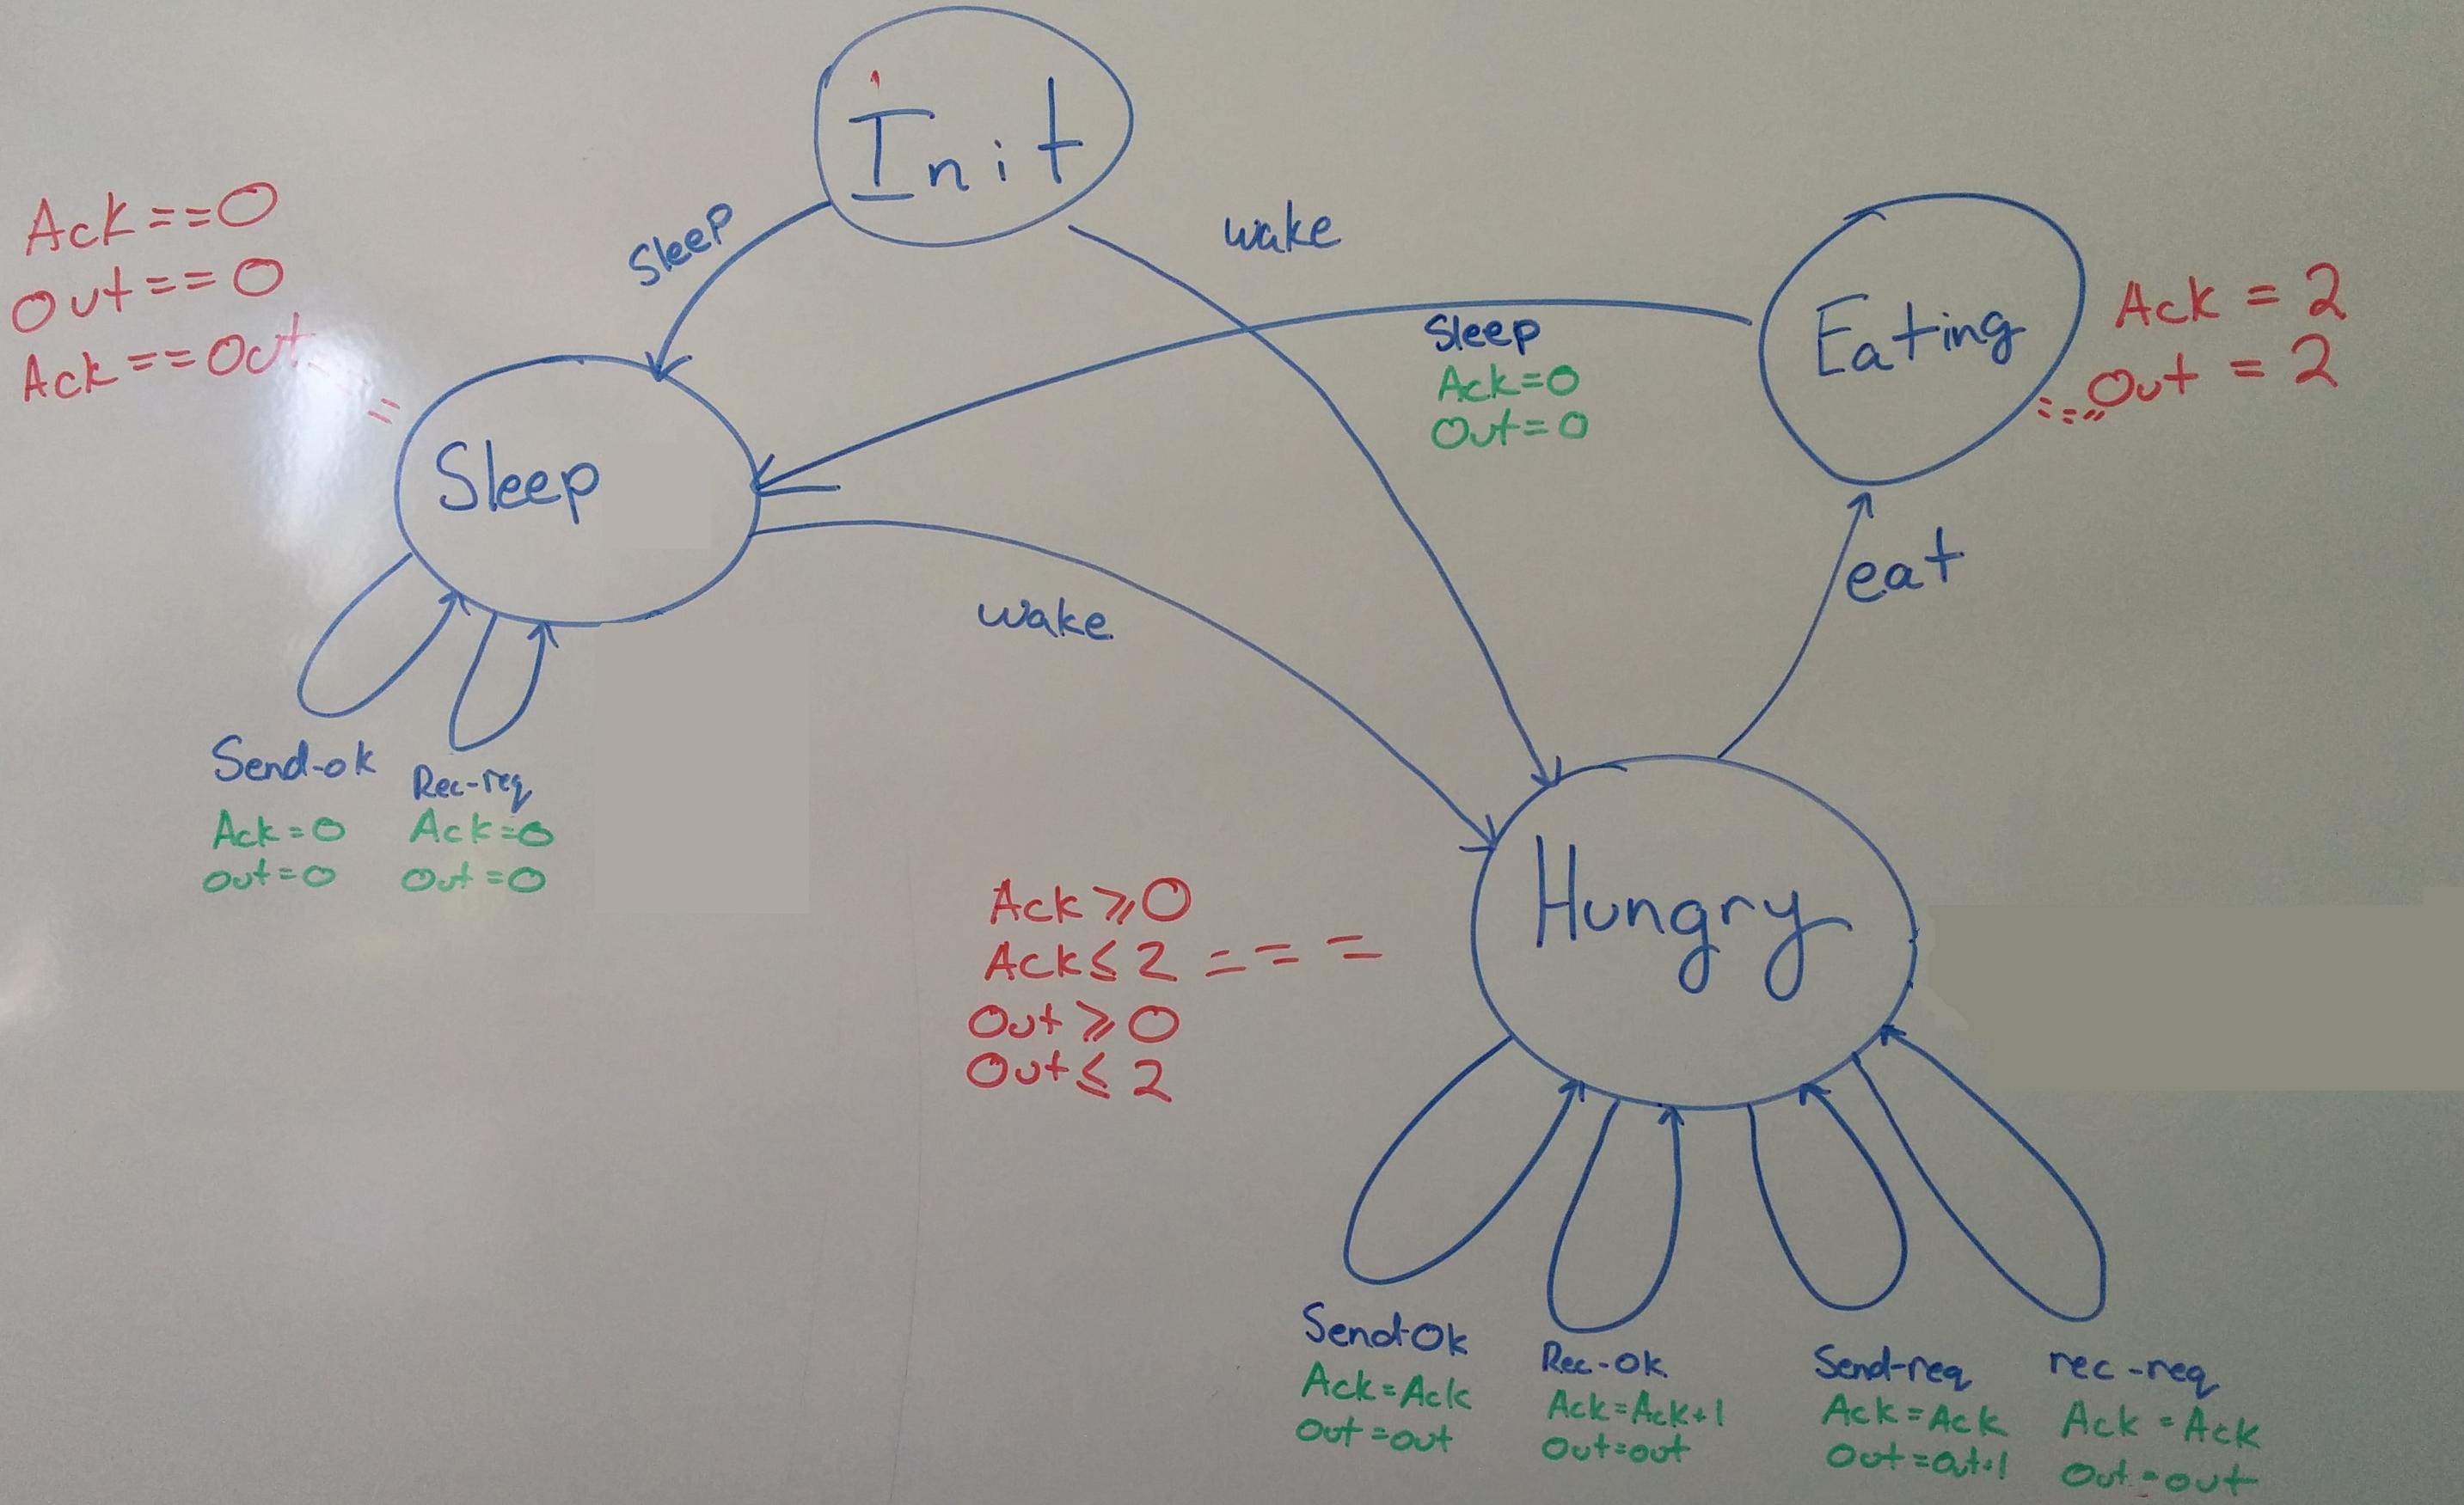
\includegraphics[width=\textwidth]{fig/relaxed}

    \caption{The dining philosophers FSM build using relaxed state matching.
    Only the $state$ variable is matched on, while $OutstandingRequests$
    ($out$), and $AcksReceived$ ($Ack$) are not matched on. Constraints in
    \textcolor{red}{red} Are invariants inferred on nodes of the FSM.
    Operations in \textcolor{green}{green} are transition operations inferred
    using SMT guided program synthesis.
    \label{fig:relaxedfsm}
    }

\end{figure*}


\subsection{Runtime}

Our runtime executes replicated versions of the inferred state machine.
Each machine can send and receive messages to any other machine, and execute
local events. The number of state machines to execute is a user defined
parameter. More machines increase runtime, but may detect subtle bugs reliant
on complicated multi machine state. Algorithm ~\ref{alg:runtime} overview our
runtime engine.

\begin{algorithm}
    \caption{Runtime Algorithm}
    \label{alg:runtime}
    \KwData{$Replication, Depth, Model, Conditions$}
    \KwResult{Condition Violating Traces}
    \While{$Depth \geq 0$}{
        $eventQueue \gets GenEvents(Model,Replication)$ \\
        \While{$\neg eventQuene.Empty()$}{
            $ApplyEvent(eventQueue.Pop())$
            $CheckSafty(Conditions)$
            $CheckLiveness(Conditions)$
            $Recurse(Replication,Depth--,Model,Conditions)$
        }
    }
\end{algorithm}

Initially all machines are set to an empty initial state $\perp$. All valid events are
generated at the beginning of the main runtime loop. A valid event is the set
of all outgoing edges of all the current state of all nodes. Each event is
added to an event queue and is applied systematically. Three kinds of events can
be applied at runtime.

\begin{itemize}

    \item\emph{Local Event} A local event transitions a single node from one state to another.

    \item\emph{Send Event} A send event generates a message, which is placed on an outstanding message list

    \item\emph{Receive Event} A receive event consumes a message. Two conditions
        exist for receiving messages, droppable, and undroppable. Droppable
        message can be consumed by any machine in any state, if no transition
        exists for the message, the state of the received machine does not
        change. Undroppable messages are only delivered to machines which are in
        a state with a transition corresponding to the message being
        received~\cite{yang_modist_nsdi09}.

\end{itemize}


Messages are consumed by only a single node. As our search is performed
systematically, all permutations of message delivery are eventually explored. 

While executing a trace of variables is maintained. Variables are updated during
each state transition. If the state transitioned into is exactly matched,
runtime variables are assigned the value of the state. Otherwise the operations
determined by constraint solving are applied to the variables.

The runtime environment has a holistic view of the system, and is therefore
able to check safety predicates at all times. Predicates defined by a user
specification, such as only one machine may enter the critical section at a
time, or at least one node has a token, are checked on a per variable basis.

As of writing this document no specification language has been chosen to
specify safety and liveness properties. A common way to specify safety properties
are as regular expressions on events, and states~\cite{5727765}, as well as
\textbf{Pos}/\textbf{Def} global predicates. Liveness properties are typically
encoded as LTL or CTL formula. As the proposed analysis technique generates
traces, and has full observation of generated execution, all specifications
should theoretically be valid input. For the purposes of this project checkers
will be designed to be plugable to support, a variety of specification
languages.

Liveness conditions are checked using techniques developed by
~\cite{Garg:2014:MAS:2580115.2580404}. If a periodic pattern is found in a
distributed execution, ie if at two points in an execution, the state of the
system is exactly the same, the events between the two states can periodically
execute forever (given non random liveness guarantees). If exact states are
revisited during runtime, and a liveness condition is not met over the interval
between matching states, a liveness violation is reported.

\subsection{Violations \& false positive reduction}

The result of simulating is a set of traces on which a safety or liveness
violation occurred. Traces contain vector time stamps for simulated events,
which are formatted to be visualized by ShiViz, to aid in
debugging~\cite{Abrahamson_sheddinglight}. Traces generated using \textbf{State
Matching} and \textbf{Event Matching} are guarantees bugs, the traces of which
can be traversed to identify the root cause of the bug. 

Traces generated using \textbf{Relaxed State Matching} and \textbf{Relaxed
Event Matching} may be false positives. These traces are approximately ordered by
their likelihood to be false positives. Each simulated trace (containing
simulated variable values at runtime) is analyzed by Daikon. Using Daikons
Invariant Difference tool the count of invariant violations generated by the
simulated execution can be determined. Traces which violate the minimum count
of invariants are reported to the user first, as they are least likely to have
diverged from the systems real behavior.


